\section{Consultas ao serviço de resolução de nomes DNS}

\subsection{Usando os registos do tipo A, identifique os endereços IPv4 dos servidores mail.uminho.pt e
www.ualg.pt? Qual o servidor de nomes que a sua máquina está a usar?}

\begin{figure}[h!]
    \centering
    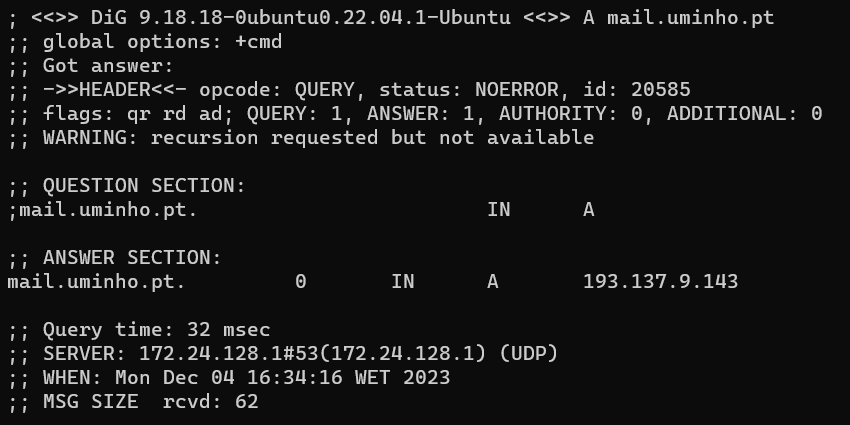
\includegraphics[width=1\textwidth]{images/ex1.mail.png}
    \caption{\label{fig:comando}Output do comando \textit{dig A mail.uminho.pt}}
\end{figure}

\begin{figure} [h!]
    \centering
    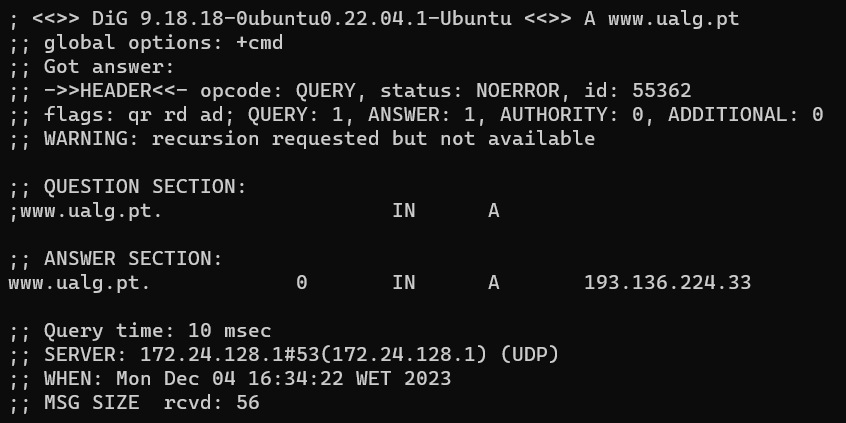
\includegraphics[width=1\textwidth]{images/ex1.ualg.png}
    \caption{\label{fig:comando1}Output do comando \textit{dig A www.ualg.pt}}
\end{figure}

\begin{figure} [h!]
    \centering
    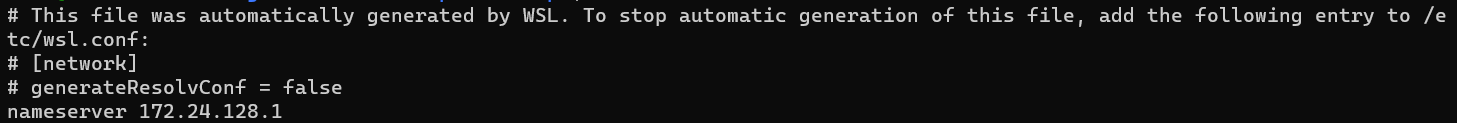
\includegraphics[width=1\textwidth]{images/ex1.resolv.png}
    \caption{\label{fig:comando2}Output do comando \textit{cat /etc/resolv.conf}}
\end{figure}


\begin{itemize}
    \item O endereço IPv4 do servidor \textit{mail.uminho.pt} é \textit{193.137.9.143}.
    \item O endereço IPv4 do servidor \textit{www.ualg.pt} é \textit{193.136.224.33}.
    \item O servidor de nomes utilizado pela sua máquina é \textit{172.24.128.1}.
\end{itemize}

O servidor de nomes utilizado pela máquina é, na verdade, uma \textit{bridge} para a 
minha máquina principal, uma vez que estou a usar wsl2. O servidor de nomes utilizado 
pela máquina principal é: 
\textit{193.137.16.65}, \textit{193.137.16.145} e \textit{193.137.16.75}

\begin{figure} [h!]
    \centering
    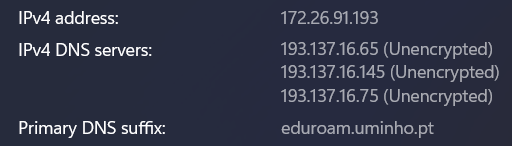
\includegraphics[width=1\textwidth]{images/ex1.windows.png}
    \caption{\label{fig:windows}IPv4 DNS do servidor de nomes da máquina principal}
\end{figure}

\subsection{Usando os registos do tipo PTR, efetue uma query para 
143.9.137.193.in-addr.arpa. O que permitiu identificar esta query?}

\begin{figure} [h!]
    \centering
    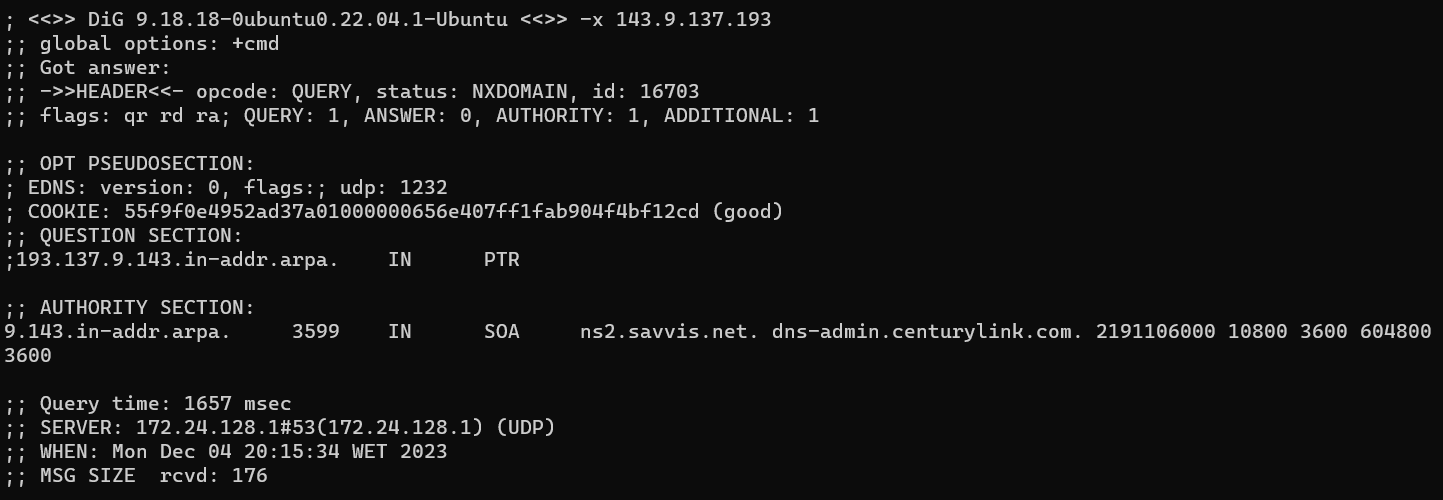
\includegraphics[width=1\textwidth]{images/ex2.143arpa.png}
    \caption{\label{fig:comando3}}Output do comando \textit{dig -x 143.9.137.193}
\end{figure}


A consulta PTR para \texttt{143.9.137.193.in-addr.arpa} resultou em 
um status de \texttt{NXDOMAIN} (não encontrado), indicando que não há 
um registro PTR associado a esse endereço IP. A resposta também 
inclui informações sobre a autoridade, mostrando que o domínio 
\texttt{9.143.in-addr.arpa} tem um registro SOA associado.


\subsection{Certas aplicações fazem uso do reverse DNS, como, por exemplo, o traceroute. Experimente fazer
traceroute (tracert no Windows) para router-di.uminho.pt, ao mesmo tempo que captura o tráfego gerado
com o Wireshark. Comente a diferença observada, em termos de tráfego DNS gerado, entre usar a opção
com e sem resolução de nomes (-n no Linux, -d no Windows). Perante o observado, diga qual a utilidade
que o reverse DNS oferece ao traceroute?}

\begin{figure} [h!]
    \centering
    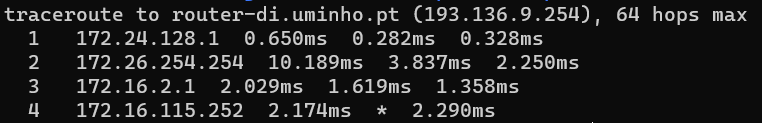
\includegraphics[width=1\textwidth]{images/ex3.traceroute.png}
    \caption{\label{fig:comando4}}Output do comando \textit{traceroute router-di.uminho.pt}
\end{figure}

O comando \texttt{traceroute} foi executado para o destino 
\texttt{router-di.uminho.pt} com o endereço IP \texttt{193.136.9.254}. 
Os resultados mostram o tempo de resposta (em milissegundos) para cada 
salto no caminho até o destino. No quarto salto, houve uma perda de 
pacotes indicada pelo asterisco (*).

\begin{enumerate}
    \item \textbf{Primeiro Salto (172.24.128.1):}
        \begin{itemize}
            \item Tempo de resposta: 0.650ms, 0.282ms, 0.328ms.
        \end{itemize}
    
    \item \textbf{Segundo Salto (172.26.254.254):}
        \begin{itemize}
            \item Tempo de resposta: 10.189ms, 3.837ms, 2.250ms.
        \end{itemize}
    
    \item \textbf{Terceiro Salto (172.16.2.1):}
        \begin{itemize}
            \item Tempo de resposta: 2.029ms, 1.619ms, 1.358ms.
        \end{itemize}
    
    \item \textbf{Quarto Salto (172.16.115.252):}
        \begin{itemize}
            \item Tempo de resposta: 2.174ms, * (perda de pacotes), 2.290ms.
        \end{itemize}
  \end{enumerate}
  
  A perda de pacotes no quarto salto pode indicar uma interrupção 
  temporária na comunicação ou congestionamento na rede nesse ponto 
  específico. O aumento no tempo de resposta nos saltos subsequentes 
  pode ser causado por várias razões, como a distância física, 
  congestão de rede ou configuração específica dos \textit{routers}.
  

\subsection{Usando o registo NS:}

\begin{itemize}
    \item Para o domínio "tecnico.ulisboa.pt." (tamanho do pacote de resposta: 381 bytes):


    \begin{verbatim}
tecnico.ulisboa.pt.     0       IN      NS      ns2.tecnico.ulisboa.pt.
tecnico.ulisboa.pt.     0       IN      NS      a.ul.pt.
tecnico.ulisboa.pt.     0       IN      NS      ns1.tecnico.ulisboa.pt.
a.ul.pt.                0       IN      A       194.117.0.150
ns1.tecnico.ulisboa.pt. 0       IN      A       193.136.128.1
ns2.tecnico.ulisboa.pt. 0       IN      A       193.136.128.2
a.ul.pt.                0       IN      AAAA    2001:690:21c0:a::150
ns1.tecnico.ulisboa.pt. 0       IN      AAAA    2001:690:2100:1::53:1
ns2.tecnico.ulisboa.pt. 0       IN      AAAA    2001:690:2100:1::2
\end{verbatim}

    \item Para o domínio "ulisboa.pt." (tamanho do pacote de resposta: 444 bytes):


    \begin{verbatim}
ulisboa.pt.             0       IN      NS      ns1.tecnico.ulisboa.pt.
ulisboa.pt.             0       IN      NS      ns2.tecnico.ulisboa.pt.
ulisboa.pt.             0       IN      NS      a.ul.pt.
ulisboa.pt.             0       IN      NS      b.ul.pt.
a.ul.pt.                0       IN      A       194.117.0.150
b.ul.pt.                0       IN      A       194.117.1.150
ns1.tecnico.ulisboa.pt. 0       IN      A       193.136.128.1
ns2.tecnico.ulisboa.pt. 0       IN      A       193.136.128.2
a.ul.pt.                0       IN      AAAA    2001:690:21c0:a::150
b.ul.pt.                0       IN      AAAA    2001:690:21c0:b::150
ns1.tecnico.ulisboa.pt. 0       IN      AAAA    2001:690:2100:1::53:1
ns2.tecnico.ulisboa.pt. 0       IN      AAAA    2001:690:2100:1::2
\end{verbatim}

    \item Para o domínio "pt." (tamanho do pacote de resposta: 658 bytes):


    \begin{verbatim}
pt.                     0       IN      NS      d.dns.pt.
pt.                     0       IN      NS      ns.dns.br.
pt.                     0       IN      NS      e.dns.pt.
pt.                     0       IN      NS      a.dns.pt.
pt.                     0       IN      NS      ns2.nic.fr.
pt.                     0       IN      NS      b.dns.pt.
pt.                     0       IN      NS      h.dns.pt.
pt.                     0       IN      NS      g.dns.pt.
pt.                     0       IN      NS      c.dns.pt.
a.dns.pt.               0       IN      A       185.39.208.1
b.dns.pt.               0       IN      A       194.0.25.23
c.dns.pt.               0       IN      A       204.61.216.105
d.dns.pt.               0       IN      A       185.39.210.1
e.dns.pt.               0       IN      A       193.136.192.64
g.dns.pt.               0       IN      A       193.136.2.226
h.dns.pt.               0       IN      A       194.146.106.138
ns.dns.br.              0       IN      A       200.160.0.5
ns2.nic.fr.             0       IN      A       192.93.0.4
a.dns.pt.               0       IN      AAAA    2a04:6d80::1
b.dns.pt.               0       IN      AAAA    2001:678:20::23
c.dns.pt.               0       IN      AAAA    2001:500:14:6105:ad::1
d.dns.pt.               0       IN      AAAA    2a04:6d82::1
e.dns.pt.               0       IN      AAAA    2001:690:a00:4001::64
g.dns.pt.               0       IN      AAAA    2001:690:a80:4001::100
\end{verbatim}

    \item Para o domínio "." (tamanho do pacote de resposta: 966 bytes):


    \begin{verbatim}
.                       0       IN      NS      e.root-servers.net.
.                       0       IN      NS      d.root-servers.net.
.                       0       IN      NS      a.root-servers.net.
.                       0       IN      NS      l.root-servers.net.
.                       0       IN      NS      g.root-servers.net.
.                       0       IN      NS      b.root-servers.net.
.                       0       IN      NS      h.root-servers.net.
.                       0       IN      NS      j.root-servers.net.
.                       0       IN      NS      f.root-servers.net.
.                       0       IN      NS      i.root-servers.net.
.                       0       IN      NS      m.root-servers.net.
.                       0       IN      NS      c.root-servers.net.
.                       0       IN      NS      k.root-servers.net.
a.root-servers.net.     0       IN      A       198.41.0.4
b.root-servers.net.     0       IN      A       170.247.170.2
c.root-servers.net.     0       IN      A       192.33.4.12
d.root-servers.net.     0       IN      A       199.7.91.13
e.root-servers.net.     0       IN      A       192.203.230.10
f.root-servers.net.     0       IN      A       192.5.5.241
g.root-servers.net.     0       IN      A       192.112.36.4
h.root-servers.net.     0       IN      A       198.97.190.53
i.root-servers.net.     0       IN      A       192.36.148.17
j.root-servers.net.     0       IN      A       192.58.128.30
k.root-servers.net.     0       IN      A       193.0.14.129
l.root-servers.net.     0       IN      A       199.7.83.42
m.root-servers.net.     0       IN      A       202.12.27.33
a.root-servers.net.     0       IN      AAAA    2001:503:ba3e::2:30
b.root-servers.net.     0       IN      AAAA    2801:1b8:10::b
\end{verbatim}

\end{itemize}


\subsubsection{Identifique os servidores de nomes definidos para os 
domínios: “tecnico.ulisboa.pt.”, “ulisboa.pt.”, “pt.” e “.” (root).}

\begin{enumerate}
    \item \textbf{tecnico.ulisboa.pt.:}
        \begin{itemize}
            \item ns2.tecnico.ulisboa.pt.
            \item a.ul.pt.
            \item ns1.tecnico.ulisboa.pt.
        \end{itemize}
    \item \textbf{ulisboa.pt.:}
        \begin{itemize}
            \item ns1.tecnico.ulisboa.pt.
            \item ns2.tecnico.ulisboa.pt.
            \item a.ul.pt.
            \item b.ul.pt.
        \end{itemize}
    \item \textbf{pt.:}
        \begin{itemize}
            \item d.dns.pt.
            \item ns.dns.br.
            \item e.dns.pt.
            \item a.dns.pt.
            \item ns2.nic.fr.
            \item b.dns.pt.
            \item h.dns.pt.
            \item g.dns.pt.
            \item c.dns.pt.
        \end{itemize}
    \item \textbf{. (root):}
        \begin{itemize}
            \item e.root-servers.net.
            \item d.root-servers.net.
            \item a.root-servers.net.
            \item l.root-servers.net.
            \item g.root-servers.net.
            \item b.root-servers.net.
            \item h.root-servers.net.
            \item j.root-servers.net.
            \item f.root-servers.net.
            \item i.root-servers.net.
            \item m.root-servers.net.
            \item c.root-servers.net.
            \item k.root-servers.net.
        \end{itemize}
\end{enumerate}


\subsubsection{Perante a informação obtida, diga, justificando, se os servidores de nomes de diferentes domínios
podem coexistir numa mesma máquina física.}

Os resultados indicam que os servidores de nomes para diferentes 
domínios estão hospedados em máquinas distintas. No entanto, apenas 
com os registros NS, não podemos afirmar conclusivamente se estão em 
máquinas físicas separadas. Para uma conclusão mais precisa, seria 
necessário verificar informações adicionais, como endereços IP e 
configurações específicas.


\subsubsection{Encontra domínios geridos por servidores de nomes localizados em redes IP distintas? Se sim,
apresente esses domínios e diga qual a vantagem resultante desse procedimento?}

Sim, é possível identificar domínios geridos por servidores de nomes 
localizados em redes IP distintas. Por exemplo, ao observar os 
servidores de nomes para o domínio "pt.", notamos que eles estão 
distribuídos em várias redes IP. Isso é uma prática comum para 
garantir redundância e maior robustez na infraestrutura de DNS. 
Alguns desses domínios são:

\begin{itemize}
    \item d.dns.pt
    \item ns.dns.br
    \item e.dns.pt
    \item a.dns.pt
    \item ns2.nic.fr
    \item b.dns.pt
    \item h.dns.pt
    \item g.dns.pt
    \item c.dns.pt
\end{itemize}

A vantagem de ter servidores de nomes em redes IP distintas está na 
resiliência do sistema. Se uma rede ou servidor falhar, outros ainda 
podem responder às consultas DNS, garantindo a disponibilidade 
contínua dos serviços.


\subsection{Usando o registo SOA:}

\subsubsection{Identifique o servidor DNS primário definido para os domínios: “tecnico.ulisboa.pt.”,
“ulisboa.pt.”, “pt.” e “.” (root).}

\begin{enumerate}
    \item \textbf{tecnico.ulisboa.pt.:}
        \begin{itemize}
            \item ns2.tecnico.ulisboa.pt.
        \end{itemize}
    \item \textbf{ulisboa.pt.:}
        \begin{itemize}
            \item ns1.tecnico.ulisboa.pt.
        \end{itemize}
    \item \textbf{pt.:}
    \begin{itemize}
        \item d.dns.pt.
    \end{itemize}
    \item \textbf{. (root):}
    \begin{itemize}
        \item a.root-servers.net.
    \end{itemize}
\end{enumerate}

\subsubsection{Quais são os servidores secundários dos domínios “tecnico.ulisboa.pt.” e “ulisboa.pt.”?
Justifique.}

\begin{enumerate}
    \item \textbf{tecnico.ulisboa.pt.:}
        \begin{itemize}
            \item a.ul.pt.
            \item ns1.tecnico.ulisboa.pt.
        \end{itemize}
    \item \textbf{ulisboa.pt.:}
        \begin{itemize}
            \item ns2.tecnico.ulisboa.pt.
        \end{itemize}
\end{enumerate}


Servidores secundários são configurados para armazenar cópias de 
zonas DNS e fornecer redundância e resistência a falhas. No caso:

\begin{itemize}
    \item Para "tecnico.ulisboa.pt.", a.ul.pt. e ns1.tecnico.ulisboa.pt. atuam como servidores secundários.
    \item Para "ulisboa.pt.", ns2.tecnico.ulisboa.pt. é o servidor secundário.
\end{itemize}

\subsubsection{Em que difere o servidor primário de um servidor secundário? Qual o significado dos parâmetros
temporais associados ao servidor primário?}

\textbf{Servidor Primário:}
\begin{itemize}
    \item Contém a cópia principal e autoritativa da zona DNS.
    \item Tem a autoridade final sobre a zona.
    \item Atualizações são feitas diretamente no servidor primário.
\end{itemize}


\textbf{Servidor Secundário:}
\begin{itemize}
    \item Mantém uma cópia secundária (réplica) da zona DNS.
    \item Obtém atualizações do servidor primário periodicamente.
    \item Serve como backup e distribui a carga de consulta.
\end{itemize}

\textbf{Parâmetros temporais associados ao servidor primário:}
\begin{itemize}
    \item \textbf{SOA (Start of Authority):}
        \begin{itemize}
            \item 2191106000: Número de série da zona.
            \begin{itemize}
                \item Incrementa a cada modificação.
            \end{itemize}
            \item 10800: Tempo de espera padrão (3 horas) antes de tentar novamente uma transferência de zona falhada.
            \item 3600: Tempo de espera entre tentativas de transferência de zona.
            \item 604800: Tempo máximo que um servidor secundário espera por uma transferência de zona antes de expirar o registro SOA.
            \item 3600: Tempo de vida padrão para registros negativos (1 hora).
        \end{itemize}
\end{itemize}

\subsection{Usando o registo MX}
\subsubsection{Quais são os servidores de email do domínio “tecnico.ulisboa.pt.”?}

Utilizando o comando dig MX tecnico.ulisboa.pt, obtemos os seguintes servidores de email:
\begin{itemize}
    \item 51 smtp1.tecnico.ulisboa.pt.
    \item 10 smtp.tecnico.ulisboa.pt.
    \item 61 smtp2.tecnico.ulisboa.pt.
\end{itemize}

\subsubsection{A que sistema são preferencialmente entregues as mensagens dirigidas a
geral@tecnico.ulisboa.pt?}

As mensagens sao preferencialmente entregues ao sistema de maior prioridade, isto e, os de menor numero a esquerda do nome do servidor de email, logo as mensagens seriam entregues ao servidor smtp.tecnico.ulisboa.pt, no caso deste estar indisponivel, a mensagem seria entao entregue ao seguintes, por ordem, smtp1.tecnico.ulisboa.pt e por fim smtp2.tecnico.ulisboa.pt.

\subsection{A resposta obtida a uma query pode ser classificada como autoritativa ou não-autoritativa.}
\subsubsection{Qual a diferença fundamental entre ambos os tipos de resposta?}

A diferença fundamental entre ambos os tipos de resposta é que uma resposta autoritativa é uma resposta que vem diretamente do servidor DNS que contém a informação sobre o domínio, enquanto que uma resposta não-autoritativa é uma resposta que vem de um servidor DNS que não contém a informação sobre o domínio, mas que obteve essa informação de um servidor DNS autoritativo.
Logo enquanto a resposta nao autoritativa pode conter informação desatualizada, a resposta autoritativa contém sempre a informação mais atualizada.

\subsubsection{Usando o seu default DNS server, que tipos de resposta obtém se efetuar queries aos registos
MX para identificar os servidores de email dos domínios “ulisboa.pt.” e “uminho.pt.”?
Experimente e justifique os tipos de respostas obtidos.}

\begin{figure}[h!]
    \centering
    \subfloat[\centering ULisboa]{{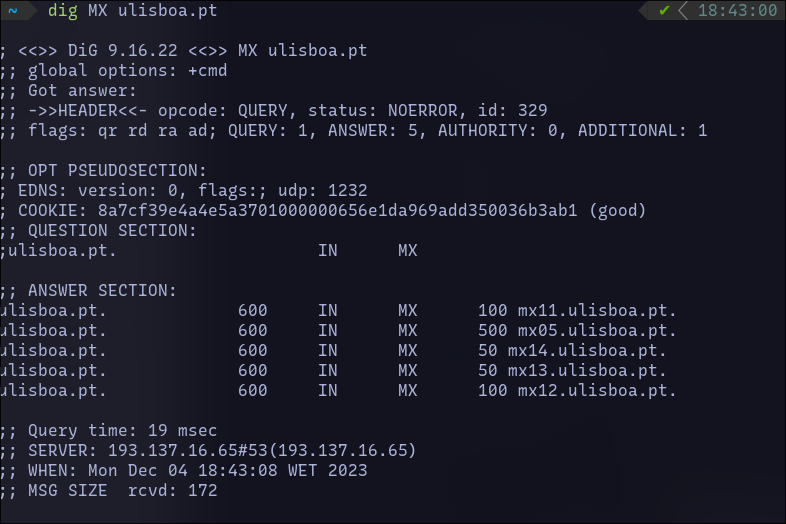
\includegraphics[width=5cm]{images/ulisboa.png} }}
    \qquad
    \subfloat[\centering UMinho]{{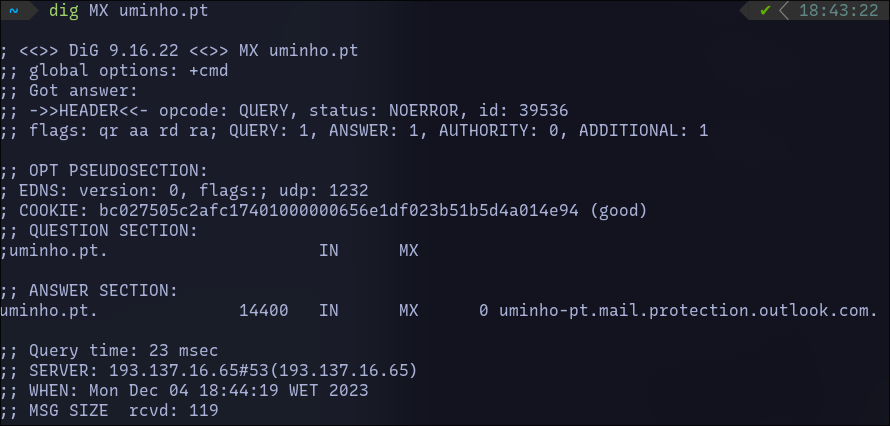
\includegraphics[width=5cm]{images/uminho.png} }}
\end{figure}